\begin{frame}[fragile]{Implementation}{STL Algorithm}
    STL provides:
    \begin{itemize}
        \item std::inclusive\_scan
        \item std::exclusive\_scan
    \end{itemize}
    \vspace{10pt}
    Essentially equivalent to:\\
    
     \begin{lstlisting}[language=C++, frame=single, gobble=4]
     float sum = 0;
     for(size_t i =0; i<N; i++)
     {
         sum += input[i];
         output[i] = sum;
     }
     \end{lstlisting}
    \begin{center} $\Rightarrow$ Sequential to a fault! \end{center}
 
\end{frame} 

\begin{frame}{Implementation}{Alternatives}
    Alternatives to STL:
    \begin{itemize}
        \item OpenMP: scan pragma
        \item TBB: parallel\_scan function
    \end{itemize}
    Alternative Algorithms:
    \begin{itemize}
     \item Up-Down Sweeping Scan
     \item Tiled Scan
    \end{itemize}
\end{frame} 

\begin{frame}{Up-Down Sweep}
\todo{UpDown description}
\end{frame}

\begin{frame}{Up-Down Sweep}{Schema Inclusive}
 \begin{figure}
  \centering
  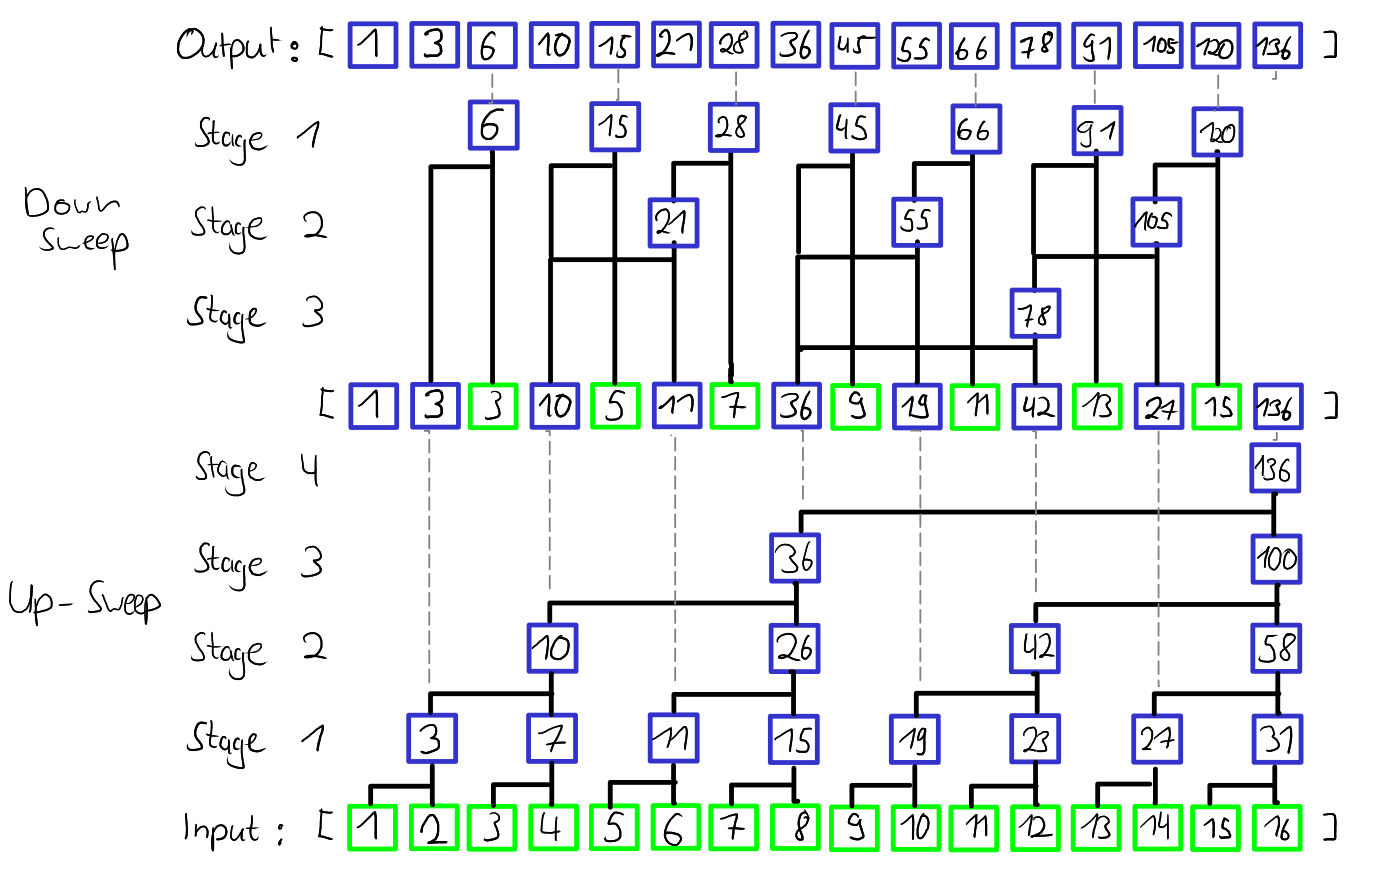
\includegraphics[width=0.85\textwidth]{wiki/InclusiveUpDown}
 \end{figure}
\end{frame}

\begin{frame}{Up-Down Sweep}{Schema Exclusive}
 \begin{figure}
  \centering
  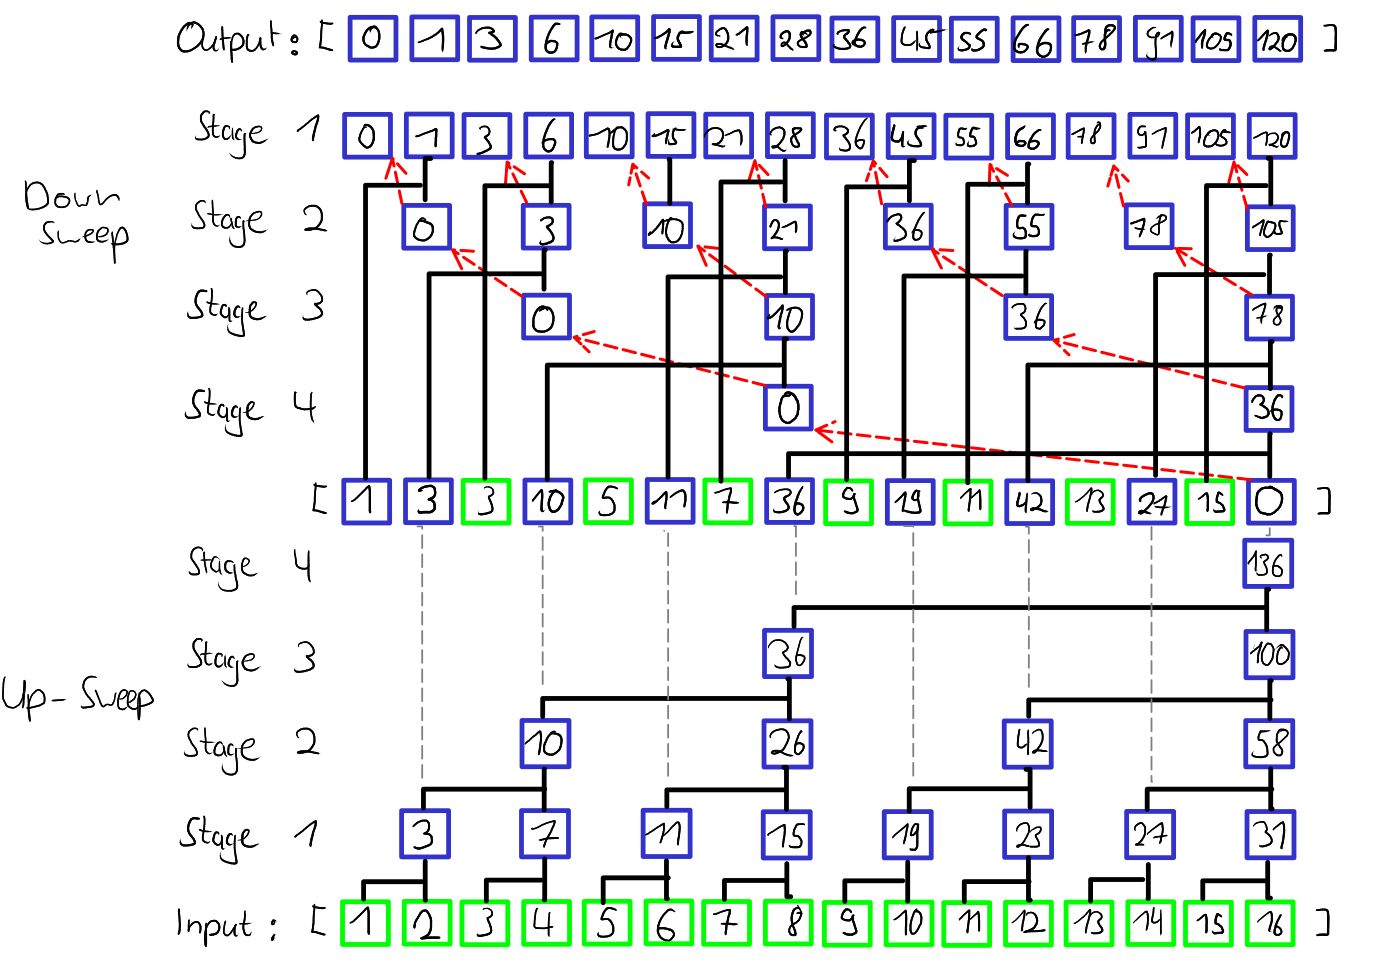
\includegraphics[width=0.85\textwidth]{wiki/ExclusiveUpDown}
 \end{figure}
\end{frame}
